\documentclass[10pt,fleqn,a4paper]{jsarticle}
\usepackage[dvipdfmx]{graphicx,color}
\usepackage{ascmac,amsmath,amssymb,amstext}
\usepackage{tikz,multicol,float,tikz-3dplot}
\usetikzlibrary{positioning,intersections,calc,arrows.meta,math,angles}
\usepackage{zogeny,ceo,comment}
\newcommand{\ans}[1]{\mbox{\boldmath{$#1$}}}
\renewcommand{\baselinestretch}{1.3} 
\tdplotsetmaincoords{60}{110}%{xy平面からどれだけ上にいるか(90度から-90度)}{z軸中心にどれだけ左右に回転するか}
\begin{document}
\begin{itembox}
[r]{\Mondai\kagil $\theta の範囲に注意せよ$\kagir(青山学院大)}
$tを0\leq t\leq\pi を満たす実数とし,xy平面上の放物線\\
\hspace{0.5cm}C:y=x^2-2(2\sin t)x+\sin t\cos t\\
の頂点を\mathrm{P}とおくとき,以下の問いに答えよ.\\
\Shomon 点\mathrm{P}の座標をtを用いて表せ.\\
\Shomon 放物線Cとx軸の正の部分が異なる2点で交わるようなtの値の範囲を求めよ.\\
\Shomon tが0\leq t\leq\pi の範囲を動くとき,点\mathrm{P}のyの最大値と最小値を求めよ.また,そのときのtの値を求めよ.$
\end{itembox}
\kangaekata\\
よくある典型的な解の配置問題です.$\kakkosan で少々方針を決めかねるかも知れませんが,合成で普通に解きましょう$.\\
\kai\\
$\kakkoichi$\indent $f(x)=x^2-2(2\sin t)x+\sin t\cos tとおくと,\\
\indent f'(x)=2x-2(2\sin t)なので,$点Pの座標は,$\kotaee{(2\sin t,-4\sin^2t+\sin t\cos t)}\\\\
\kakkoni\indent 「Cがx軸の正の部分で異なる2点と交わる.」\doti \begin{cases}
    点\mathrm{P}のx,y座標が共に正\\
    F(0)>0
\end{cases}\\\\
\doti \begin{cases}
    \sin t>0\\
    -4\sin^2t+\sin t\cos t>0\\
    \sin t\cos t>0
\end{cases}\doti\begin{cases}
    \sin t>0\\
    \cos t>0\\
    \sin t(4\sin t-\cos t)<0
\end{cases}\\\\
\doti\kotaee{0<t<\dfrac{\pi}{2}}$\\\\
\kakkosan\indent $g(t)=-4\sin^2t+\sin t\cos とおくと,半角の公式より,g(t)=-4\cdot\dfrac{1-\cos2t}{2}+\sin t\cos t と書ける.\\
これを整理すると,g(t)=\dfrac{1}{2}\p{\sin2t+4\cos2t}-2と書くことができるので,これを更に合成することにより,\\
\indent g(t)=\dfrac{1}{2}\p{\sqrt{17}\sin\p{2t+\phi}}-2\cdots\maruichi\indent \p{ただし,\phi は
\begin{cases}
    \cos\phi=\dfrac{1}{\sqrt{17}}\\
    \sin\phi=\dfrac{4}{\sqrt{17}}
\end{cases}を満たす角である.}\\
ここで、2t+\phi の取りうる値の範囲は,\phi が第一象限の角であることから,\dfrac{\pi}{2}<2t+\phi<2\pi+\dfrac{\pi}{2}なので,\\
\kotaee{\begin{cases}
    \max{g(t)}=\dfrac{\sqrt{17}}{2}-2\\
    \min{g(t)}=-\dfrac{\sqrt{17}}{2}-2
\end{cases}}である.$


\newpage
\begin{itembox}
[r]{$\Mondai\kagil 見た目に惑わされてはいけない \kagir$(中央大)}
数列$\B{a_n}を,条件a_1=1と漸化式\\
\hspace{0.5cm}a_{n+1}=(n+1)a_n+(n-1)!\indent(n=1,2,3,\cdots)\\
によって定める.ただし,0!=1である.また,数列\B{b_n}を\\
\hspace{0.5cm}b_n=\dfrac{a_n}{n!}\\
で定める.このとき,以下の問いに答えよ.\\
\Shomon b_1,b_2,b_3を求めよ.答えのみ記せば良い.\\
\Shomon \B{b_n}の満たすべき漸化式を求めよ.また,\B{b_n}の一般項を求め\B{a_n}の一般項を求めよ.\\
\Shomon nを自然数とする.次の等式を証明せよ.\\
\hspace{0.5cm}\wa{K=1}{n}2^{k-1}a_k=2^nn!-1\\$
\end{itembox}
\kangaekata\\
誘導に乗ることができればどの小問も優しいです.教科書レベルの問題になります.ただ,\ans{\kakkoni}に関しては,$b_n=\dfrac{a_n}{n!} を
b_nの式だけで表したいのでa_{n+1}の漸化式を両辺(n+1)!で割り算すれば\ans{b_n}の階差数列になります.$\\\\
\kai\\
$\kakkoichi\indent $ $b_1=\dfrac{a_1}{1!}=\ans{1}\\\\
\hspace{0.2cm}b_2=\dfrac{a_2}{2!}=\dfrac{2\cdot a_1+0!}{2\cdot1}=\ans{\dfrac{2}{3}}\\\\
\hspace{0.2cm}b_3=\dfrac{a_3}{3!}=\dfrac{3\cdot a_2+1!}{3\cdot2\cdot1}=\kotaee{\dfrac{5}{3}}\\\\
\kakkoni\indent a_{n+1}=(n+1)a_n+(n-1)!の両辺を(n+1)!で割ることにより,$
\begin{center} $\dfrac{a_{n+1}}{(n+1)!}=\dfrac{a_n}{n!}+\dfrac{1}{n(n+1)}(n\geq1)$\end{center}
\begin{center}$\doti \kotaee{b_{n+1}=b_n+\dfrac{1}{n(n+1)}(n\geq1)}$\end{center}
$\Y b_n=b_1+\wa{k=1}{n-1}\p{\dfrac{1}{k}-\dfrac{1}{k+1}}=1-\tint{\dfrac{1}{k}}{1}{n}\\
\hspace{1.7cm}=1-\p{\dfrac{1}{n}-1}=2-\dfrac{1}{n}(n\geq1)\\
これは、n=1のときも成立する.\\
\Y\kotaee{a_n=\p{2-\dfrac{1}{n}}n!(n\geq1)}\\\\
\kakkosan\indent \kakkoni より,\kakkosan における示すべき等式は次のように書ける.$
\begin{center}
    $\wa{k=1}{n}2^{k-1}\cdot\p{2-\dfrac{1}{k}}k!=2^nn!-1\cdots\cdots\maruichi $
\end{center}
このことより,\\
\indent $2^{k-1}\p{2-\dfrac{1}{k}}k!=2^{k-1}\B{2k!-(k-1)!}\\\\
\hspace{0.5cm}=2^k\cdot k!-2^{k-1}(k-1)!\indent\temarkua\ans{差分型!(階差型!)}\\\\
\Y \wa{k=1}{n}\B{2^k\cdot k!-2^{k-1}(k-1)!}=\tint{2^{k-1}\cdot(k-1)!}{1}{n+1}\\\\
\hspace{0.5cm}=2^n\cdot n!-(1\cdot0!)=2^nn!-1\hspace{1cm}\ans{(証明終わり)}$
\newpage
\begin{itembox}
    [r]{\Mondai \kagil 人は見かけによらない\kagir(津田塾大-文系)}
    次の問いに答えよ.\\
    $\kakkoichi$ 袋の中に赤玉$5$個,白玉$3$個の合計$8$個の玉が入っている.この中から一度に$3$個の玉を
    取り出したとき,赤玉が$1$個,白玉が$2$個取り出される確率を求めよ.\\
    $\kakkoni$ 袋の中に赤玉$n個,白玉9個の合計n+9個の玉が入っている.この中から一度に3個の玉を
    取り出したとき,赤玉が1個,白玉が2個取り出される確率P_nを求めよ.ただし,nは自然数とする.$\\
    $\kakkosan$ $\kakkoni のP_nについて,\dfrac{P_{n+1}}{P_n}>1を満たすnを全て求めよ.$\\
    $\kakkoshi$ $\kakkoni のP_nについて,P_nを最大にするnを求めよ.$
\end{itembox}
\kangaekata\\
愚直に確率を計算するだけです.計算ミスに気をつけましょう.\\\\
\kai\\
$\kakkoichi\indent \dfrac{{}_5C_3\times{}_3C_1}{{}_8C_3}=\kotaee{\dfrac{15}{56}}\\\\
\kakkoni\indent P_n=\dfrac{{}_nC_1\times{}_9C_2}{{}_{n+9}C_3}=\kotaee{\dfrac{216n}{(n+9)(n+8)(n+7)}}\\\\
\kakkosan\indent P_{n+1}=\dfrac{216(n+1)}{(n+10)(n+9)(n+8)}より,$
\begin{center}
$\dfrac{P_{n+1}}{P_n}=\dfrac{216(n+1)/(n+10)(n+9)(n+8)}{216n/(n+9)(n+8)(n+7)}=\dfrac{(n+1)(n+7)}{n(n+10)}$
\end{center}
なので,\\
    \indent$\dfrac{P_{n+1}}{P_n}>1\doti\dfrac{(n+1)(n+7)}{n(n+10)}>1\\\\
    \indent\doti\dfrac{(n+1)(n+7)-n(n+10)}{n(n+10)}>0\\\\
    \indent\doti-\dfrac{2n-7}{n(n+10)}>0\\\\
    \indent\doti\dfrac{2n-7}{n+10}<0\\\\
    \indent\doti(2n-7)n(n+10)<0\cdots\cdots\maruichi \\
    \maruichi が満たす領域を図示すると次図の斜線部である.$
    \newpage
    \begin{center}
        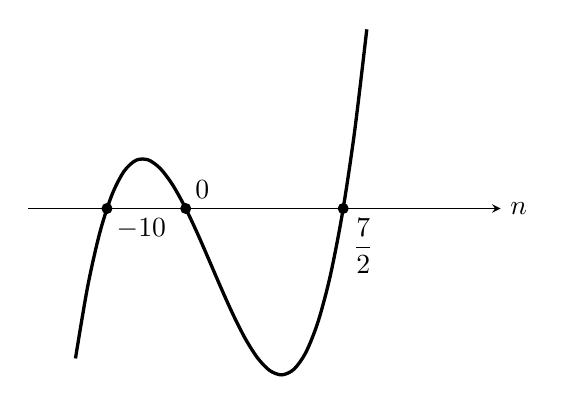
\begin{tikzpicture}[scale=1]
            \draw[->,>=stealth](-2,0)--(4,0)node[right]{$n$};
            \draw[smooth,very thick,domain=-1.4:2.3]plot (\x,{\x*\x*\x-\x*\x-2*\x});
            \coordinate(A)at(-1,0);
            \coordinate(B)at(0,0);
            \coordinate(C)at(2,0);
            \node[below right]at(A){$-10$};
            \node[above right]at(B){$0$};
            \node[below right]at(C){$\dfrac{7}{2}$};
            \fill(A)circle(2pt);
            \fill(B)circle(2pt);
            \fill(C)circle(2pt);

        \end{tikzpicture}
    \end{center}
上図の斜線部が$\maruichi$が満たす領域である.$nが自然数であることから,0<n<\dfrac{7}{2}を満たす自然数nを求めればよいので,求めるnは
\kotaee{n=1,2,3}$\\\\
$\kakkoshi\indent\maruichi より, $
\begin{center}
$P_1<P_2<P_3<P_4>P_5>P_6\cdots $
\end{center}
なので,$P_nを最大にするようなnは、\kotaee{n=4}$
$\p{\because\heiki{\dfrac{P_{n+1}}{P_n}>1\narabaa n<4 }{\dfrac{P_{n+1}}{P_n}<1\narabaa n>4}}$

\newpage
\begin{itembox}
    [r]{\ba{1}.\kagil そろそろ見飽きた三平方の整数問題\kagir(一橋大)}
    以下の問いに答えよ.\\
    $\Shomon 整数a,b,cがa^2+b^2=c^2を満たすとき,abは4の倍数であることを示せ.\\
    \Shomon 3辺の長さがすべて整数で,そのうちの一辺の長さが2025である三角形の面積は
    162の倍数であることを示せ.$

\end{itembox}
\kangaekata\\
$\kakkoichi はもうお手のものですね.\ans{背理法}でいきましょう.\\
\kakkoni \tokeiichi a=2025 またはb=2025\tokeini c=2025 の二つの場合に限られるとうことは見抜けるでしょう.ポイントは,
\ans{2025=3^4\cdot5^2,162=3^4\cdot2と因数分解できる.}ということです.$\\
\kai\\
$\kakkoichi 「a,bが4の倍数」\doti 「a\godo0\kmod{4}またはb\godo0\kmod{4}」\\
ここで,\begin{cases}
    a\negodo0\kmod{4}\\
    b\negodo0\kmod{4}
\end{cases} と仮定すると,ある整数k,lを用いて,
   \begin{cases}
    a=4k+1\\
    b=4l+1
\end{cases}と書くことができる.\\
このことより,\\
 a^2+b^2=16k^2+16l^2+8k+8l+2\godo2\kmod{4}\\
\Y c^2\godo2\kmod{4}\eqnum{E1}\\
ここで,一般の整数nについて,法を4とすると,下表のような結果を得る.$\\
\begin{center}
    \begin{tabular}{|c||c|c|c|c|}
        \hline
        $n\kmod{4}$ & $0$ & $1$ & $2$ & $3$\\
        \hline
        $n^2\kmod{4}$ & $0$ & $1$ & $0$ & $9\godo1$\\
        \hline
    \end{tabular}
\end{center}
上表より,$\kakkoichi は,矛盾である.\\
\Y abは4の倍数である.\hspace{0.5cm}\ans{(証明終わり)}$\\
$\kakkoni  今,直角三角形の3辺の長さを大小関係をつけてa,b,c(a\leq b\leq c),直角三角形の面積をSとおくことにする.\\
\kakkoichi からabの少なくとも一方は4の倍数であるから,1辺の長さが2025である直角三角形は次の2つの場合に限定される.$
\newpage
$\underline{\tokeiichi a=2025 または b=2025 のとき,}\\
「S=\dfrac{1}{2}\times2025\times a または S=\dfrac{1}{2}\times2025\times b」\doti 「S=\dfrac{1}{2}3^4\cdot5^2\times4k または S=\dfrac{1}{2}3^4\cdot5^2\times4l」\\
\doti 「S=\dfrac{1}{2}324\times25\times k または S=\dfrac{1}{2}324\times25\times l」 \doti 「S\godo0\kmod{162}」$\\
$\underline{\tokeini c=2025のとき,}\\
 a^2+b^2=\p{2025}^2=\p{3^4\cdot5^2}^2\godo0\kmod{3}なので,適当な整数p,qを用いて\begin{cases}
    a=3p\\
    b=3q
\end{cases}と書くことができる.\\
\Y a^2+b^2=9p^2+0q^2=\p{3^4\cdot5^2}^2\doti p^2+q^2=\p{3^3\cdot5^2}^2\\
\narabaa p^2+q^2\godo0\kmod{3}\\
\Y p\godo q\godo0\kmod{9}なので,a\godo b\godo0\kmod{9}であるから,c=2025のときの直角三角形の面積Sは,S=\dfrac{1}{2}\times81\times4kと書ける.\\
\Y S\godo0\kmod{162}\\
以上により,題意は示された.\hspace{0.5cm}\ans{(証明終わり)}$
\newpage
\begin{itembox}
    [r]{\ba{2}\kagil \ans{束}という概念\kagir(一橋大・改)}
    $tを実数とし,座平面上において\\
      x^2+y^2-1-t\p{4x+2y-10}=0\\
     で表される図形C_tを考える.このとき,以下の問いに答えよ.\\
     \kakkoichi  t=1のときC_1を図示せよ.\\
     \kakkoni  C_tの半径が1以上4以下になるための条件をtを用いて表せ.\\
     \kakkosan  C_tが\kakkoni で求めた範囲を動くとき,Cが通過してできる領域を求め,図示せよ.$

\end{itembox}
\kangaekata\\
$\kakkoichi  半径の正負に応じて円の方程式がどのような図形を表すか覚えていますか.その確認です.\\
円の方程式(x-a)^2+(y-b)^2=rとおく.$
\begin{center}
    $\ans{\begin{cases}
      r>0\doti (a,b)中心の円\\  
      r=0\doti 点(a,b)\\
      r<0\doti 図形を描かない
    \end{cases}}$
\end{center}
$\kakkoni  xとyでまとめて,定数項を右辺に寄せてやればいいですね.\\
\kakkosan  通過領域の典型的な問題です.通過領域は次のような同値変形をすることによりときます.\\
\ans{「ある点(X,Y)が通過領域Wに入る」\doti 「x=X,y=Yを代入した方程式を満たすようなtが少なくと一つ存在する.」}$\\
\kai\\
$\kakkoichi  t=1のとき,C_1:x^2+y^2-4x-2y-1+10=0\doti (x-2)^2+(y-1)^2=-9\\
\Y \ans{描く図形はない.}\\
\kakkoni  x^2+y^2-1-t(4x+2y-10)=0\doti x^2-4tx+y^2-2ty+10t-1=0\\
      \doti (x-2t)^2+(y-t)^2=5t^2-10t+1\\
これより,\\
 「C_tの半径が1以上4以下」\doti1\leq\sqrt{5t^2-10t+1}\leq4\\
\doti \begin{cases}
    t(t-2)\geq0\\
    (t+1)(t-3)\leq0
\end{cases}\doti\begin{cases}
    t\geq2\vee t\leq0\\
    -1\leq t\leq3
\end{cases}\doti\kotaee{2\leq t\leq3\vee-1\leq t\leq0}$\\
\newpage
$\kakkosan  Cが通過する領域をW,\kakkoni で得られたtの範囲を\maruichi とおく.$
\begin{align*}
   (X,Y)\in W&\doti (X,Y)がWを通るようなtが\maruichi の範囲に少なくとも一つ存在する.\\
   &\doti\exists t\in\maruichi,X^2+Y^2-1-t(4X+2Y-10)=0\doti\exists t\in\maruichi, t=\dfrac{X^2+Y^2-1}{4X+2Y-10}\\
   &\doti\begin{aligned}
    \begin{cases}
        \p{X^2+Y^2-1}\B{\p{X-4}^2+\p{Y-2}^2-1}\geq0\cdots\maruni\\
        \B{\p{X+2}^2+\p{Y+1}^2-16}\B{\p{X-6}^2+\p{Y-3}^2-16}\leq0\cdots\marusan
    \end{cases}
   \end{aligned}
\end{align*}
このことより,$\maruni と\marusan の零領域を描いて領域を図示すると下図を得る.(\temarkua \ans{かわりばんこの法則を使う!!})$\\

\begin{center}
    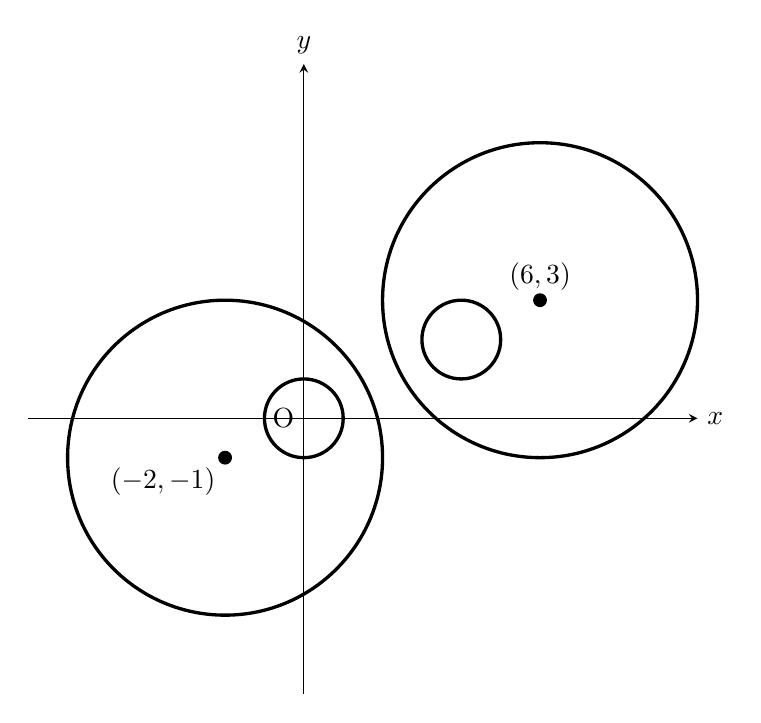
\begin{tikzpicture}[scale=0.5]
        \draw[->,>=stealth](-7,0)--(10,0)node[right]{$x$};
        \draw[->,>=stealth](0,-7)--(0,9)node[above]{$y$};
        \draw[very thick](0,0)circle[radius=1];
        \draw[very thick](4,2)circle[radius=1];
        \draw[very thick](-2,-1)circle[radius=4];
        \draw[very thick](6,3)circle[radius=4];
        \coordinate[label=left:O](O)at(0,0);
        \coordinate(A)at(6,3);
        \fill[black](A)circle(5pt);
        \node[above]at(6,3){$(6,3)$};
        \coordinate(B)at(-2,-1);
        \fill[black](B)circle(5pt);
        \node[below left]at(B){$(-2,-1)$};

    \end{tikzpicture}
\end{center}
\newpage
\begin{itembox}
    [r]{$\ba{3}.相反方程式(東京医大・改)$}
    $4次方程式\\
     x^4+11x^3+31x^2+11x+1=0\cdots\asta\\
    について考える.このとき,次の問いに答えよ.\\
    \kakkoichi y=x+\dfrac{1}{x}とおくことにより\asta をyで表せ.\\
    \kakkoni  4次方程式\asta の4つの解を\alpha,\beta,\gamma,\delta とおくとき,次のそれぞれの
    値を求めよ.\\
     \tokeiichi  \dfrac{1}{\alpha}+\dfrac{1}{\beta}+\dfrac{1}{\gamma}+\dfrac{1}{\delta}\\
     \tokeini  \alpha^2+\beta^2+\gamma^2+\delta^2\\
     \tokeisan  \alpha^3+\beta^3+\gamma^3+\delta^3$

\end{itembox}
\kangaekata\\
相反方程式の基本的な問題です.\\
$\kakkoichi  \asta の両辺をx^2で割ることにより,yで表すことができます.\\
\kakkoni  \kakkoichi  の誘導を踏襲しましょう.yについて解くと,二つの解が得られます.\\
ということは、\ans{(y-(解1))(y-(解2))=0と因数分解することができる!}$\\
\kai\\
$\kakkoichi \asta の両辺をx^2で割ることにより,$
\begin{align*}
    &x^2+11x+31+\dfrac{11}{x}+\dfrac{1}{x^2}=0\\
    &\doti \p{x+\dfrac{1}{x}}^2-2+11\p{x+\dfrac{1}{x}}+31=0\\
    &\doti \kotaee{y^2+11y+29=0}
\end{align*}
$\kakkoni  \kakkoichi より,yついて解くと,y=\dfrac{-11\pm\sqrt{5}}{2}なので,$\\
\begin{align*}
    &y^2+11y+29=0\doti\p{y-\dfrac{-11\pm\sqrt{5}}{2}}\p{y-\dfrac{-11-\sqrt{5}}{2}}=0\\
    &\doti\p{x+\dfrac{1}{x}-\dfrac{-11\pm\sqrt{5}}{2}}\p{x+\dfrac{1}{x}-\dfrac{-11-\sqrt{5}}{2}}=0\\
    &\doti\p{x^2+\dfrac{11-\sqrt{5}}{2}x+1}\p{x^2+\dfrac{11+\sqrt{5}}{2}x+1}=0
\end{align*}
\newpage
ここで,$\alpha,\beta,\gamma,\delta は\asta の異なる4解なので,\\
x^2+\dfrac{11-\sqrt{5}}{2}x+1=0\doti\p{x-\alpha}\p{x-\beta}=0\cdots\maruichi $\\
        かつ\\
$x^2+\dfrac{11+\sqrt{5}}{2}x+1=0\doti\p{x-\gamma}\p{x-\delta}=0\cdots\maruni \\
としても,一般性を失わない.\\
\Y \maruichi と\maruni に解と係数の関係を用いて,\\
  \begin{cases}
    \alpha+\beta=\dfrac{-11+\sqrt{5}}{2}\\
    \alpha\beta=1
 \end{cases}かつ \begin{cases}
    \gamma+\delta=-\dfrac{11+\sqrt{5}}{2}\\
    \gamma\delta=1
 \end{cases}と書くことができる.\\\\
 \tokeiichi$ \begin{align*}  \dfrac{1}{\alpha}+\dfrac{1}{\beta}+\dfrac{1}{\gamma}+\dfrac{1}{\delta}
 &=\dfrac{\alpha+\beta}{\alpha\beta}+\dfrac{\gamma+\delta}{\gamma\delta}\\
 &=\dfrac{-11+\sqrt{5}-11-\sqrt{5}}{2}\\
 &=\kotaee{-11}
 \end{align*}
$\tokeini$  \begin{align*}
    \alpha^2+\beta^2+\gamma^2+\delta^2&=\p{\alpha+\beta}^2-\alpha\beta+\p{\gamma+\delta}^2-2\gamma\delta\\
    &=\dfrac{1}{4}\p{\sqrt{5}-11}^2-2+\dfrac{1}{4}\p{\sqrt{5}+11}^2-2\\
    &=\dfrac{1}{4}\p{10-22\sqrt{5}+22\sqrt{5}+121\times2}-4\\
    &=\dfrac{1}{4}\times\p{252}-4=\kotaee{59}
\end{align*}
\newpage
$\tokeisan$  \begin{align*}
    \alpha^3+\beta^3+\gamma^3+\delta^3&=\p{\alpha+\beta}^3-3\alpha\beta\p{\alpha+\beta}+\p{\gamma+\delta}^3
    -3\gamma\delta\p{\gamma+\delta}\\
    &=\dfrac{1}{8}\p{-11+\sqrt{5}}^3-3\cdot\p{\dfrac{-11+\sqrt{5}}{2}}-\dfrac{1}{8}\p{11+\sqrt{5}}+
    3\cdot\p{\dfrac{11+\sqrt{5}}{2}}\\
    &=\dfrac{3}{2}\p{11+\sqrt{5}+11-\sqrt{5}}+\dfrac{1}{8}\B{\p{\sqrt{5}-11}^3-\p{\sqrt{5}+11}^3}\\
    &=33+\dfrac{1}{8}\p{-11^3\cdot2-3\cdot5\cdot11\times2+3\sqrt{5}\cdot11^2-3\sqrt{5}\cdot11^2}\\
    &=33-\dfrac{2\cdot11}{8}\p{121+15}\\
    &=33-\dfrac{11}{4}\cdot136\\
    &=33-11\cdot34\\
    &=-374+33\\
    &=\kotaee{-341}
\end{align*}
\newpage
\begin{itembox}
    [r]{\ba{1}.\kagil 束と円 \kagir(同志社大)}
    $tを正の実数とし,xy平面において,不等式\\
     x^2+y^2+4t^2+\dfrac{9}{t^2}\leq20+\left|4tx+\dfrac{6}{t}y\right|\\
    の表す領域をD_tの面積をS(t)とする.このとき,次の問いに答えよ.\\
    \kakkoichi  不等式x\leq|y|の表す領域を図示せよ.\\
    \kakkoni  不等式x^2+y^2\leq7+4x+6yの表す領域を図示せよ.\\
    \kakkosan  t=1のとき,領域D_1をxy平面に図示せよ.\\
    \kakkoshi  S(t)が最小となるtの値を求めよ.$

\end{itembox}
\kangaekata\\

\noindent\kai\\



\newpage

\begin{itembox}
    [r]{\ba{2}.\kagil ベクトルの標準的な問題\kagir(お茶の水女子大)}
    平面において$\mathrm{OA}=3,\mathrm{OB}=2,\mathrm{AB}=\sqrt{7}である三角形OABを考える.直線\mathrm{AB}
    上の点\mathrm{P}を線分\mathrm{OP}と直線\mathrm{AB}が垂直になるようにとる.\\
    \vec{a}=\Vec{OA},\Vec{b}=\vec{OB}として次の問いに答えよ.\\
    \kakkoichi  内積\vec{a}\cdot\vec{b}の値を求めよ.\\
    \kakkoni  ベクトル\vec{OP}を\vec{a},\vec{b}を用いて表せ.\\
    \kakkosan  線分\mathrm{AB}上に\Kaku{POQ}=\dfrac{\pi}{6}となる点\mathrm{Q}がただ一つあることを示し,
    ベクトル\Vec{OQ}を\vec{a},\vec{b}を用いて表せ.$
\end{itembox}

\noindent\kangaekata\\

\noindent\kai\\








\newpage
\begin{itembox}
    [r]{\ba{3}.\kagil ガウス記号の取り扱い\kagir(慶応大・改)}
    $実数xについて,\lbrack x\rbrack をxを超えない最大の整数とする.今,正の整数nに対して,
    数列\B{a_n}をa_n=n-\lbrack\sqrt{n}\rbrack^2+1と定義するとき以下の問いに答えよ.\\
    \kakkoichi  a_n=10となる最も小さなnを求めよ.\\
    \kakkoni  \wa{i=1}{27}a_iを計算せよ.\\
    \kakkosan  \wa{i=1}{n^2}a_iを計算せよ.$

\end{itembox}
\kangaekata\\


\noindent\kai\\


\end{document}